\chapter{Introduction}


Understandably, the restoration after a fault is an essential task in the operation of power systems. The \emph{restoration process}\index{restoration process} returns the system back to normal operation after any combination of system components have been lost as a result of a fault. Restoration has traditionally been performed by qualified technicians, assisted by guidelines developed by utilities using knowledge gained through experience. But now, in the era of computers and big data, it is natural to try to find a way to model this problem computationally and to solve it using more advanced techniques. Over the course of this thesis, we will both model algorithmically the current technique used by the technicians and find a new method that can exploit the information of the environment that we have available.

In this chapter, we will analyze the power grid of the city of Trieste, with all its components, and how the faults that happen are handled. Specifically, we will focus on faults occurring on the medium voltage power grid. In fact, this is what we are going to model in subsequent chapters. To this day, the company managing the grid relies on specialized technicians who, using their experience, try to restore the electricity to all users as quickly as possible. We will see how they operate, and we will understand the problems that may arise.


\section{Power grid elements}

The power grid of Trieste is handled by AcegasApsAmga S.p.A. (\acrshort{aaa}), an Italian company based in Trieste and subject to the direction and coordination of Hera S.p.A., also called Hera Group, which is a multiutility company based in Bologna, Italy. Hera operates in the sale and distribution of gas, water, energy, and waste disposal in some Italian northeastern provinces. It is also responsible for the infrastructures, on which it operates a technical and administrative management. AcegasApsAmga does the same, but is restricted to some municipalities of Veneto, Friuli-Venezia Giulia, and in the Balkans.

As part of the electricity supply chain,
which is the sequence of production steps that start from the raw material and arrive at the finished product, % <- Matteo would remove this
\acrshort{aaa} also deals with the transmission and the distribution of electricity. The \emph{transmission} consists of the transport of electricity on the national power grid in high -- or very high --- voltage, to deliver it in the regional distribution networks to local distributors to which end users are connected. The \emph{distribution} consists of transporting electricity on local networks for delivery to end customers, and in those activities related to all accessory operations for the connection of end users. The company is responsible for ensuring the safety and continuity of supply, providing for the management and maintenance of the entire electricity network and the systems connected to it. In particular, the company must also handle and resolve any blackouts deriving from faults that may occur on the power line, something called \emph{restoration process}\index{restoration process}.

We will now describe Trieste's power grid, mainly the one in medium voltage --- since it is the one we are interested in, and all its elements.  The electricity produced from different primary sources of energy is transmitted in high or very high voltage to the \emph{primary substations}\index{primary substation}, an electrical system that has the function of transforming the high voltage input energy into medium voltage energy. Then, the electricity is transmitted in medium voltage to the \emph{secondary substations}\index{secondary substation}, an electrical system for transforming electrical energy from medium voltage to low voltage, and is then distributed to the users. Actually, some users like big supermarkets or malls can receive the power directly in medium voltage, and then use their transformers to convert it to low voltage.

Specifically, a substation is a complex of conductors, equipment, and machines designed to transform the voltage of the electrical lines. After being transported through the cables, the electricity arrives in the substation at the \emph{(circuit) breakers}\index{breaker}, which are electrical switches that allow to open or close a circuit, respectively stopping or allowing the power to flow. Then the power flows through a \emph{busbar}\index{busbar} (or two, depending on the substation), which is a metallic strip, or bar, used to carry and distribute the current to multiple circuits. Afterwards, it passes through a \emph{transformer}\index{transformer}, which decreases its voltage. At this point, if it is a primary substation, the electricity flows through another busbar, and finally exits the substation in medium voltage through a breaker. If it is a secondary substation, the electricity in medium voltage exits directly through the breaker to arrive at another secondary substation. There is also electricity in low voltage that exits the substation, which arrives at the final users, but since we have no interest in these elements, we will not discuss them. A \emph{single-line diagram}\index{single-line diagram} is a symbolic schematic of the components of a three-phase electric system, which uses only one line to represent all three phases. In \autoref{fig:schema-primary-substation} we can see an example of a single-line diagram of a primary substation, with a description of the main elements that we just mentioned.

\begin{figure}[t]
    \centering
    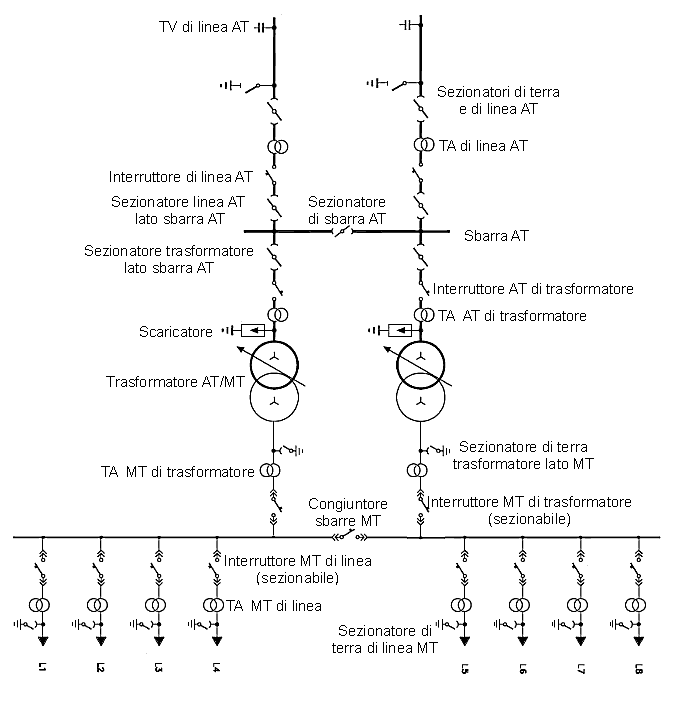
\includegraphics[width=0.8\textwidth]{chapters/figures/Schema_Unifilare_Cabina_Primaria.png}
    \caption{Example of a single-line diagram of a primary substation, with a description of the main elements (adapted from \href{https://it.wikipedia.org/wiki/Cabina_primaria}{Wikipedia}).}
    \label{fig:schema-primary-substation}
\end{figure}

\begin{figure}[ph]
    \centering
    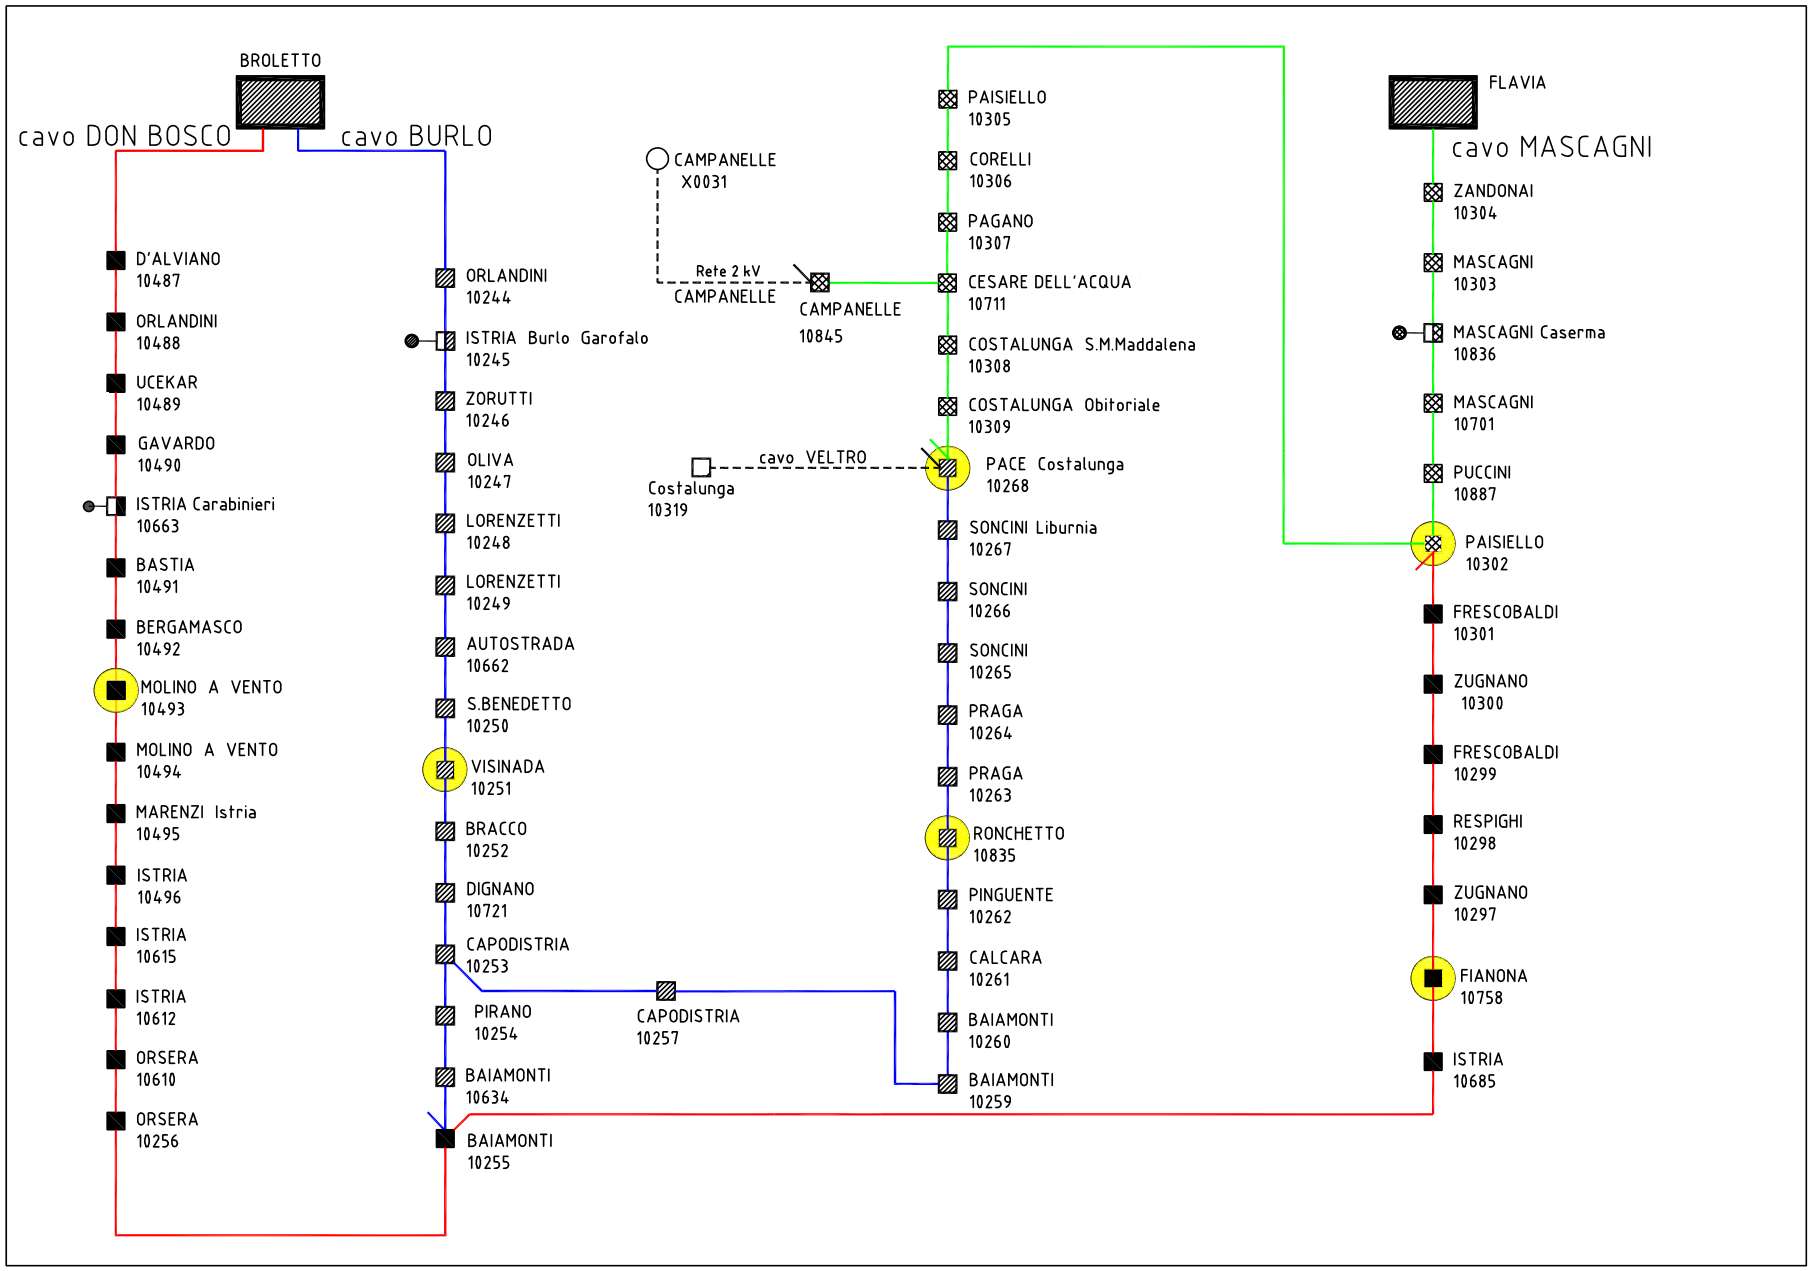
\includegraphics[scale=0.35, center]{chapters/figures/Mastrino.png}
    \caption{Electrical diagram of three power lines of Trieste's power grid, indicated with different colors. The big rectangles at the top are the two primary substations, while the small squares are the secondary substations. The yellow circles specify which are the remotely controlled substations (all the primary substations are). The hyphen which can be seen attached to some substations indicates that the breaker of that cable in that substation is open in the standard set-up. The black circles next to some secondary substations indicate the points of delivery in medium voltage.}
    \label{fig:mastrino}
\end{figure}

Instead, an \emph{electrical diagram}\index{electrical diagram} is a schematic that represents the electrical connections between the various elements of the power grid --- the primary and secondary substations and the electrical cables that connect them -- using standardized symbolic representations. The presentation of the interconnections in these diagrams does not necessarily correspond to the real arrangements, and, most importantly, the lengths of the cables are not to scale. They are mainly used to know the power supply sequence of the secondary substations in the \emph{standard set up}\index{standard set up}, which means when everything is working fine and all the faulty elements are fixed. In \autoref{fig:mastrino}, we can see an electrical diagram of three lines of Trieste's power grid, indicated with different colors. The big rectangles at the top are the two primary substations, while the small squares are the secondary substations. The yellow circles specify which are the remotely controlled substations --- note that all the primary substations are. In a \emph{remotely controlled substation}\index{remotely controlled substation}, the breakers are motorized in order to be able to be operated remotely. This happens from the \emph{remote control room}\index{remote control room}, which is also responsible for monitoring the entire network. The black circles connected to some secondary substations indicate the \emph{points of delivery}\index{point of delivery} in medium voltage, like the ones to malls or supermarkets. The hyphen that can be seen attached to some substations indicates that the breaker of that cable in that substation is open in the standard set-up, which means that the electricity doesn't flow in that substation through that cable. This derives from the fact that we have a \emph{meshed electrical grid}\index{meshed electrical grid}, which means that the power grid allows for alternative interconnection paths between any two substations, and therefore allows powering the same substation from different power grid cables, ensuring greater continuity of service. Thanks to this redundancy, after a fault, the users are reconnected in very few hours rerouting the power through other cables, while the technicians restore the damaged line, which remains deactivated and thus can be safely fixed. After everything is repaired, the power flow is brought back to the standard setup. It's worth highlighting that, however, the cost of meshed electrical grids limits their application to medium voltage transmission and distribution networks.


\section{When a failure happens}

A fault can happen for various reasons and in all possible elements of the power grid. If it is one of the elements of a substation that breaks, often it is because it is flawed, and when the technician visits that substations, they can notice it right away, and usually they just have to replace that element. If the fault happens on an electrical cable, it is usually because it is no longer perfectly isolated, for example, because the wire's insulation breaks down --- caused maybe by some workers that cut the cable while doing road works, or by some rats that chew it, or simply by the deterioration of the insulating material. This causes a short circuit since the cable is connected to the ground and allows the charge to flow through it.

What happens after a fault on the medium voltage power line has occurred? The fault creates a short circuit, so a fault current propagates backward to the primary substation, and causes the breaker in the latter to open, disconnecting all the secondary substations that were powered by that substation through this specific cable line. A \emph{fault current}\index{fault current} is a current different from the normal one, as it has different properties; first of all, it has a much higher amperage, even around $1000$ amperes (the normal one is around $50$ amperes). A substation can see if there has been a fault through the \emph{fault detectors}\index{fault detectors}: they are devices that analyze the current, and if it is a fault current, then they know that there has been a fault in some substation after this one.

The opening of the breaker and the disconnection of the substations trigger the alarm in the remote control room\index{remote control room}; at that point, the operators immediately alert the technicians, and the restoration process\index{restoration process} begins. First of all, the technicians ask the remote control room\index{remote control room} to check which fault detector detected the fault, in order to know in which segment of the power line the problem is. In this way, they are able to figure out the section of the line among two remotely controlled substations in which the fault happened. Then they proceed to remotely operate the breakers of the remotely controlled substations in order to restore the power to the substations outside this tract. For the substations after the fault, they use the power of another primary substation to power them, closing one of the breakers of the open cables: this is possible thanks to the meshed electrical grid\index{meshed electrical grid}. These operations are very fast: they take around $5$ minutes in total. After this, they are left with only a small subset of non remotely controlled substations, which the technician has to visit in person to reconnect while searching for the fault. They will be called the initially disconnected substations in subsequent chapters. This manual restoration process is the part of the problem we will focus on, modeling it computationally and searching for a better algorithm to solve it.


\section{The manual restoration process}

To this day, the technique that the technicians follow to decide which substation to visit among the initially disconnected ones is \emph{binary search}\index{binar search}, which they call \emph{bisection}\index{bisection}. This means that they go in the substation that is in the middle (considering the number of disconnected substations), or almost in the middle, depending on the ease of access to the substation and maneuvering of the breakers (which could be old and break easily). It can happen, for example, that a substation is in a bank; accessing it at night could easily take several hours, because the technician has to wait for the security service. A substation could also be located in a fenced courtyard, have a faulty door lock, or be inaccessible due to adverse weather conditions.

Once in the substation, the technician has the possibility of finding out if the fault is before or after the substation in which they currently are. This is done with two different methods, and the one to use depends on many factors, among which the length of the electrical cable and whether it is day or night. The first one, the most used, is the \emph{instrumental test}\index{instrumental test}, which consists of opening a breaker in the substation to divide the cable into two segments, and attaching a detecting device to one of them. It has a needle for the voltage and a needle for the current, and it works by measuring how much current the cable draws when applying a voltage to it. If the tension needle moves, but the current needle remains on zero, then the cable is fine; while if the tension needle stays on zero, but the current needle goes to the full scale of the instrument (the maximum amplitude the system can represent), then on this cable there is a fault. In this way, this device can tell if the fault is before or after the current substation. However, this test is only possible if the length of the cable being checked is less than $2 \, \mathrm{km}$. If the cable is too long, the technician has to go to another substation of the line and open a breaker, so to reduce the length of the cable that is being tested, and then return to the substation to actually perform the test. This procedure is typically employed during the daytime, and if there are important users connected to the line, like hospitals, police stations, or firehouses.

The second method consists in simply proceeding by trial-and-error: once in a substation, the technician opens the breaker of the cable that exits the substation and goes into the next one, and asks the remote control room to close the breaker in the primary substation, repowering the line. If the cable doesn't short circuit again, this means that the fault is after the current substation, otherwise, it is before it. A couple of remarks on this method are in order. First, this test has to be done only on the cable that has experienced the failure, not on other ones, to avoid creating a blackout for users connected to an unbroken line. Second, the technician opens the breaker of the cable that exits the substation, and not the one of the cable that enters it, because, if the power does not fail --- which means that the fault is after the current substation, this substation is already powered back on.
% Actually, if you open the breakers of the cable that enters and the fault is before the current substation, also in this case you don't have any other operation to do in this substation, but the technician prefers this method.
Third, if instead the fault is before the current substation, closing the breaker in the primary substation causes the power to fail again, which means that all the users on this entire line will be disconnected again and experience a second blackout. For this reason, this method is used only if the first one is not available, or if it is night, when there are much fewer active users, and is especially not used in presence of important users, like the ones mentioned before.
% the number of remaining cabins decreases exponentially

After having discovered if the fault is before or after the current substation, the technician can reconnect the segment of the electrical line that doesn't contain the fault. Thus, they can reconnect up to half the substations each time, so the time it takes to find the fault is in the order of the logarithm of the number of substations, and this is why the technicians use binary search. The fault is considered solved once all the users are reconnected again.

The technicians aim at reconnecting the users in the quickest way possible not only for the mere desire of offering a good service, but also for a more financial reason: each fault has an actual cost for the company. In fact, the company has to refund all the users that were disconnected. If the fault lasts more than an hour, the reimbursement that they have to pay is much higher, so it is important to act fast. Each user is refunded based on the time they have been disconnected. Thus, the cost of the fault is computed as the time each underlying user of each substation remains disconnected.

In the next chapters, we will model this problem and we will look for an algorithm that allows us to optimize the sequence of visited substations in order to minimize this cost. The algorithm has to decide in which substation the technician has to go after the one they are currently in, in order to solve the fault with the minimum cost. In fact, we will find an algorithm that can do better than just ``going halfway'', taking advantage of the information we have at our disposal.